\documentclass{sig-alt-release2}
\usepackage{url}
\usepackage{color}
\usepackage{graphics,graphicx}

\usepackage{epsfig}
\usepackage{epstopdf}

\usepackage{colortbl}
\usepackage{multirow}
\usepackage{booktabs}
\usepackage{ifthen}  

\begin{document}
\newcommand{\todo}[1]{\textcolor{red}{#1}}
%\def\newblock{\hskip .11em plus .33em minus .07em}

%\conferenceinfo{DIM3} {2010, Glasgow, UK} 
%\CopyrightYear{2010}
%\clubpenalty=10000
%\widowpenalty = 10000

\title{{Report Name}}

%\numberofauthors{1}
%\author{
%\alignauthor
%Author Names\\
%	   \affaddr{Team D}\\
%      \affaddr{Dim3}\\
%      \affaddr{Fiona Buyers, Chris James, Ryan Wells}\\
%             \email{\{1003648b, 1003019j, 1002253w \}@students.glasgow.ac.uk }
%}
\maketitle

\begin{abstract}
Provide a concise summary of the design of the application. i wish i was dead

\end{abstract}

\section{Aim of Application}

\subsection{Application Purpose}

The application is a multiplayer game stuff. When users register they will be randomly assigned to one of four factions. Within the faction the user will aim to increase not only their individual score, but the score of their faction. The user will have to buy buildings to expand their `city' and increase their population. There will be several different kinds of buildings; farms, barracks, studios and labs; and each will gain the user points in a different category (food, military, art and science, respectively) and all buildings will earn the user money. Crisis events will occur throughout the game which will cause buildings of a certain kind to become less or more effective, for example famine or war, so in order for the user to have a successful city and gain the maximum number of points, the city they have created should be fairly well balanced. More accomplised users will be able to unlock different personas when they have enough money. These personas will give the user different multipliers for each of the points categories which will affect the amount earned from each kind of building.

\subsection{Functional Requirements}

\begin{itemize}

\item The user's individual score should be tracked.

\item The individual score should affect the appropriate team's overall score.

\item Upon registration, the user should be randomly assigned a faction.

\item The amount of money a user currently has should be tracked and the user should not be allowed to buy buildings or personas that cost more than they have, and when an item is bought the amount of money possess should be altered appropriately.

\item Users should earn money and points from their current buildings at set time intervals.

\item 

\end{itemize}
 
\begin{itemize}

\item	What is the purpose of the application?

\item	Eg. The application is an academic search engine called AcaSe and is it is based upon the PuppyIR Framework\cite{glassey2011framework}, which has been used to construct other such services\cite{glassey2010fifi,elliot2010fifi}. The main purpose of this web application is to provide a customized interface to services such as Google Scholar and MS Academic Search. 

\item	What are the assumptions about the aims and objectives?

\item	Describe the design goals and objectives of the application.

\item	What are the constraints of the project?

\item	Functionality List: i.e. what is the required and desired functionality?

\item	Reflective Questions: 
\item	Is the scope of the application appropriate? 
\item	Are the design goals realistic/achievable? 
\item	How complex is the application? 
\item	Is distribution across the web appropriate? 

\end{itemize}

\section{Client Interface}

\verticalspace

the thing shows the main page of the thing which has lots of stuff, blah blah blah dribble dribble arse

\begin{figure}[!htbp]
  \caption{\textit{Main Page}}
  \begin{center}
		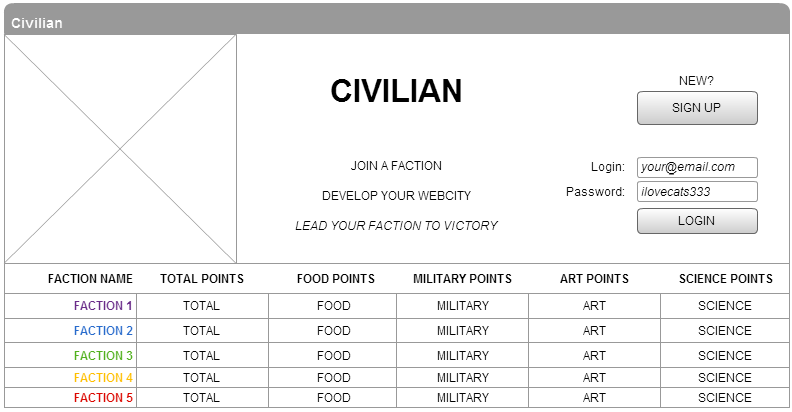
\includegraphics[scale=0.25]{img/w3.png}
  \end{center}
\end{figure}

the other one shows more stuff that is a lie.

\begin{figure}[!htbp]
  \caption{\textit{Game Page}}
  \begin{center}
		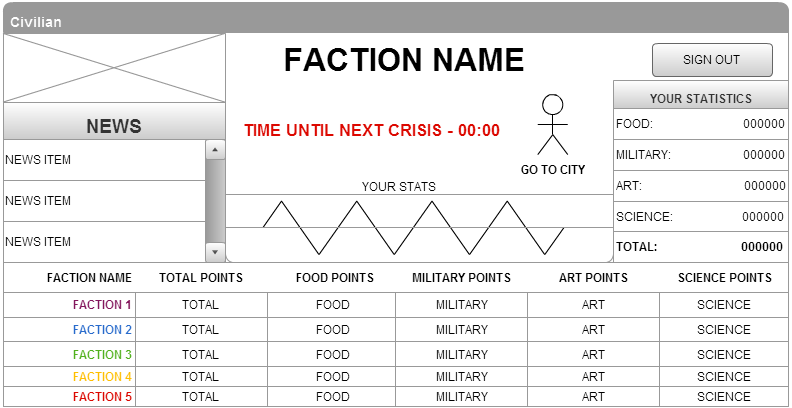
\includegraphics[scale=0.25]{img/w4.png}
  \end{center}
\end{figure}



\begin{itemize}

\item	Draw a wireframe of the user interface 

\item	this may require several wireframes depending on the complexity of the application and the interfaces

\item	Describe the user interface.

the user interface has been designed to be as simple as possible. 
there are three main screens: 
main page - options to login, register or view the current faction scores
faction scores page - shows the faction that currently has the most money, and also the greatest number of points for each of the categories - should be accessible from within the game and without logging in
game page - shows the current number of buildings each user has, displays their current amounts of points and money which will be updated after each turn. also allows the user to buy more buildings and buy different personas. 

\item	i.e. Label key input and output components: describe them.

\item	Provide a Walkthrough and explain the user interactions with application. 
\item	i.e. use cases AAAAAAAAARGH

\item	Describe the interactions associated with the dynamic components on the user interface.

\item	What calls are required to dynamically update the data on the client side?

\item	How does the user interface help the user achieve their goal, or complete their task? 

\item	Is the user interface intuitive, appealing, usable, etc?

\item	What technologies are used on the client side? 

\item	What are the reasons for your choices? i.e. what is the advantages and disadvantages of using this technology? 

\item	What other options are there? 

\end{itemize}

\section{Application Architecture}
\begin{itemize}

\item	N-Teir Architecture Diagram - chris has this

\item	i.e. data flow diagram between the interface/client, middle ware, and backend services/data repos

\item	Describe the data model i.e. what data needs to be stored or persisted by the application?

\item	What are the relationships within the data model.
\item	i.e. use ER diagram and explain. - chris 

\item	Describe the backend services used (if any).

\item	Reflective Questions: 
\item	How have you ensured that there is a separation of concerns? 
\item	What other technology could have been used instead of django? 
\item	What are the advantages of using a Web Application Framework over other technology? 
\item	And, what are the disadvantages?
\end{itemize}

\section{Message Parsing}
\begin{itemize}

\item	On the architecture diagram, Identify and label the main messages that will be parsed through the application.
\item	or alternatively (and preferably) include sequence diagrams to denote the sequence of communications parse between clients and servers.

\item	Describe the messages that are parsed back and forth through the application.

\item	For the main transactions - describe the payload of the messages 
\item	i.e. What are the contents of the messages? i.e. include sample XML, XHTML, JSON, etc of one or two messages.

\item	What is the format of the messages? 

\item	Why this format? 

\item	What other formats could be used, what are the advantages and disadvantages of these other formats?
\end{itemize}


\section{Implementation Notes}

\begin{itemize}

\item Views - What are the main views that you have implemented and what do they do?



\item URL Mapping Schema - what is your URL mapping and schema?

\item External Services  - what external services does your application include and what handlers did you include?

\item	Functionality Checklist (which functionality is completed) - everything except crises 

\item	Known Issues (what kind of works, what kind of errors to do you get)

\item What technologies have been used and are required for the application. Include a list or table of all the technologies, standards, and protocols that will be required.
\end{itemize}

\section{Reflective Summary}
{\bf For the Implementation Report Only:}
\begin{itemize}

\item	What have you learnt through the process of development? 

\item	How did the application of frameworks help or hinder your progress? 

\item	What problems did you encounter? - timing?

\item	What were your major achievements?
\end{itemize}

\section{Summary and Future Work}
\begin{itemize}

\item	Summary of application and its current state.

\item	Include a list or table of all the technologies, standards, and protocols that will be required.

\item	What are the limitations?

\item Plans for future development - crisis events, more personas and buildings.

\end{itemize}

\section{Acknowledgements}
Our thanks to the lecturers and demonstrators for their comments and suggestions. And our thanks to the peer reviewers for their feedback.
Be sincere and be specific about how others have helped your group.

\bibliographystyle{abbrv}
\bibliography{sig-proc}

\end{document}
